% Options for packages loaded elsewhere
\PassOptionsToPackage{unicode}{hyperref}
\PassOptionsToPackage{hyphens}{url}
%
\documentclass[
]{book}
\usepackage{amsmath,amssymb}
\usepackage{lmodern}
\usepackage{ifxetex,ifluatex}
\ifnum 0\ifxetex 1\fi\ifluatex 1\fi=0 % if pdftex
  \usepackage[T1]{fontenc}
  \usepackage[utf8]{inputenc}
  \usepackage{textcomp} % provide euro and other symbols
\else % if luatex or xetex
  \usepackage{unicode-math}
  \defaultfontfeatures{Scale=MatchLowercase}
  \defaultfontfeatures[\rmfamily]{Ligatures=TeX,Scale=1}
\fi
% Use upquote if available, for straight quotes in verbatim environments
\IfFileExists{upquote.sty}{\usepackage{upquote}}{}
\IfFileExists{microtype.sty}{% use microtype if available
  \usepackage[]{microtype}
  \UseMicrotypeSet[protrusion]{basicmath} % disable protrusion for tt fonts
}{}
\makeatletter
\@ifundefined{KOMAClassName}{% if non-KOMA class
  \IfFileExists{parskip.sty}{%
    \usepackage{parskip}
  }{% else
    \setlength{\parindent}{0pt}
    \setlength{\parskip}{6pt plus 2pt minus 1pt}}
}{% if KOMA class
  \KOMAoptions{parskip=half}}
\makeatother
\usepackage{xcolor}
\IfFileExists{xurl.sty}{\usepackage{xurl}}{} % add URL line breaks if available
\IfFileExists{bookmark.sty}{\usepackage{bookmark}}{\usepackage{hyperref}}
\hypersetup{
  pdftitle={Livestock Breeding and Genomics},
  pdfauthor={Peter von Rohr},
  hidelinks,
  pdfcreator={LaTeX via pandoc}}
\urlstyle{same} % disable monospaced font for URLs
\usepackage{longtable,booktabs,array}
\usepackage{calc} % for calculating minipage widths
% Correct order of tables after \paragraph or \subparagraph
\usepackage{etoolbox}
\makeatletter
\patchcmd\longtable{\par}{\if@noskipsec\mbox{}\fi\par}{}{}
\makeatother
% Allow footnotes in longtable head/foot
\IfFileExists{footnotehyper.sty}{\usepackage{footnotehyper}}{\usepackage{footnote}}
\makesavenoteenv{longtable}
\usepackage{graphicx}
\makeatletter
\def\maxwidth{\ifdim\Gin@nat@width>\linewidth\linewidth\else\Gin@nat@width\fi}
\def\maxheight{\ifdim\Gin@nat@height>\textheight\textheight\else\Gin@nat@height\fi}
\makeatother
% Scale images if necessary, so that they will not overflow the page
% margins by default, and it is still possible to overwrite the defaults
% using explicit options in \includegraphics[width, height, ...]{}
\setkeys{Gin}{width=\maxwidth,height=\maxheight,keepaspectratio}
% Set default figure placement to htbp
\makeatletter
\def\fps@figure{htbp}
\makeatother
\setlength{\emergencystretch}{3em} % prevent overfull lines
\providecommand{\tightlist}{%
  \setlength{\itemsep}{0pt}\setlength{\parskip}{0pt}}
\setcounter{secnumdepth}{5}
\usepackage{float}
\usepackage{flafter}
\usepackage{booktabs}
\usepackage{amsthm}
\usepackage{longtable}
\usepackage{array}
\usepackage{multirow}
%\usepackage[table]{xcolor}
\usepackage{wrapfig}
\usepackage{colortbl}
\usepackage{pdflscape}
\usepackage{tabu}
\usepackage{threeparttable}
\usepackage{threeparttablex}
\usepackage[normalem]{ulem}
\usepackage{makecell}

\makeatletter
\def\thm@space@setup{%
  \thm@preskip=8pt plus 2pt minus 4pt
  \thm@postskip=\thm@preskip
}
\makeatother
\ifluatex
  \usepackage{selnolig}  % disable illegal ligatures
\fi
\usepackage[]{natbib}
\bibliographystyle{apalike}

\title{Livestock Breeding and Genomics}
\author{Peter von Rohr}
\date{2021-09-30}

\usepackage{amsthm}
\newtheorem{theorem}{Theorem}[chapter]
\newtheorem{lemma}{Lemma}[chapter]
\newtheorem{corollary}{Corollary}[chapter]
\newtheorem{proposition}{Proposition}[chapter]
\newtheorem{conjecture}{Conjecture}[chapter]
\theoremstyle{definition}
\newtheorem{definition}{Definition}[chapter]
\theoremstyle{definition}
\newtheorem{example}{Example}[chapter]
\theoremstyle{definition}
\newtheorem{exercise}{Exercise}[chapter]
\theoremstyle{remark}
\newtheorem*{remark}{Remark}
\newtheorem*{solution}{Solution}
\begin{document}
\maketitle

{
\setcounter{tocdepth}{1}
\tableofcontents
}
\hypertarget{preface}{%
\chapter*{Preface}\label{preface}}
\addcontentsline{toc}{chapter}{Preface}

Livestock Breeding and Genomics is a masters course taught in the Institute of Agricultural Sciences at ETH Zurich. The aim of this course is to introduce the basic concepts of livestock breeding and genomics to the students.

\hypertarget{prerequisites}{%
\section*{Prerequisites}\label{prerequisites}}
\addcontentsline{toc}{section}{Prerequisites}

There are no explicit prerequisites for this course. All required concepts are explained during this course. Although basic knowledge in the following areas is definitely helpful for this course.

\begin{itemize}
\tightlist
\item
  \textbf{Linear Algebra}: Basic properties of and basic operations with vectors and matrices
\item
  \textbf{Statistics}: Simple linear models and least squares
\item
  \textbf{R}: Basics of how to work with data and how to do simple computations
\end{itemize}

\hypertarget{goals}{%
\section*{Goals}\label{goals}}
\addcontentsline{toc}{section}{Goals}

The following goals are taken from the teaching system at ETH. The students are able to set up design matrices, the additive genetic relationship matrix and its inverse as well as the mixed model equations to estimate BLUP breeding values. The concept of BLUP breeding values are also extended to genomic selection. All concepts introduced during this course are not only presented during the lecture, but students are expected to work with the concepts on small example problems.

\hypertarget{specific-learning-goals}{%
\subsection*{Specific Learning Goals}\label{specific-learning-goals}}
\addcontentsline{toc}{subsection}{Specific Learning Goals}

The students \ldots{}

\begin{itemize}
\tightlist
\item
  \ldots{} understand the basic concepts of livestock breeding and genomics.
\item
  \ldots{} can separate the concepts of breeding and genomics from the techniques that are important in a livestock production enterprise.
\item
  \ldots{} are familiar with the basic tools used in livestock breeding and genomics.
\item
  \ldots{} know for which problems these tools can be applied.
\item
  \ldots{} understand the genetic foundation behind the theory on which livestock breeding and genomics is based on.
\item
  \ldots{} are able to extend the genetic theory into the statistical models used in livestock breeding and genomics.
\item
  \ldots{} can extract the practical meaning of the results of the statistical analyses.
\end{itemize}

\hypertarget{exam}{%
\section*{Exam}\label{exam}}
\addcontentsline{toc}{section}{Exam}

There will be a written exam during the lecture of the last week of the semester. The exam is going to be an open-book exam. All material that seams helpful to students will be allowed. The students must solve the exams on their own. The exam is not designed to be solved in teams.

\hypertarget{lecture-notes}{%
\section*{Lecture Notes}\label{lecture-notes}}
\addcontentsline{toc}{section}{Lecture Notes}

These lecture notes contain all the relevant material for the exam. The appendix of the course notes contains two chapters, which introduce the necessary tools to work through the material of this course. Those tools consist of linear algebra and R. These chapters are mostly left to students to work through by themselves. Different students have different levels of skills in the topics of linear algebra and R. Hence not every student needs to go through the presented material at the same depth.

\hypertarget{intro-lbg}{%
\chapter{Introduction}\label{intro-lbg}}

\hypertarget{intro-lbg-terminology}{%
\section{Terminology}\label{intro-lbg-terminology}}

The terms

\begin{itemize}
\tightlist
\item
  \textbf{Livestock Breeding} and
\item
  \textbf{Animal Breeding}
\end{itemize}

are used interchangeably in this course. Although, the latter is a more general term, whereas the former focuses on livestock species, i.e.~animals which are typically present on a farm such as cattle, pig, goat and sheep. Animal breeding in general could also include pets such as dogs or cats or even zoo animals. But the very interesting topic of breeding such species is outside of the scope of this lecture and is therefore not covered in these course notes.

The term \emph{livestock breeding} is sometimes understood ambiguously. In general, most people do not differentiate between livestock breeding and animal husbandry or animal production. From a scientific point of view a \emph{Livestock Breeder} is a person who owns a number of animals from which he or she selects parent animals and uses a designed mating scheme to achieve a certain goal with the offspring animals. Most commonly known are breeders of pet animals such as dogs, cats or birds which follow individual breeding goals which focus on specific phenotypic appearance or on special behavioral traits. Around the end of the \(19^{th}\) century, livestock breeders have realized that they have to collaborate in breeding associations to be able to effectively select parent animals from a large breeding population. This allowed them to achieve more robust selection responses in shorter amounts of time, especially for livestock species with long generation intervals such as cattle and horse. This development is nicely documented by the archive of Swiss agricultural history available at \url{https://www.histoirerurale.ch/afaahr/}. In summary, livestock breeders are primarily interested in selecting parent animals with the best genetic potential to produce offspring animals that are closer to a breeding goal. From an economic point of view the sale of breeding animals to other farmers makes an important contribution to the economic result of the farm.

In contrast to livestock breeding, livestock production focuses on the aspects of keeping animals on farms to produce goods that can be sold. Nowadays, the goods produced by farm animals are mostly used in human nutrition. Due to the focus on the production aspects, the economic result of the production process is determined by the difference between monetary revenue for the products and the costs that are caused by the production of the goods.

Depending on the livestock species, the separation between breeding and production is more pronounced. In pigs, most farms are specialized into either breeding farms or production farms. Most cattle farms run as mixed operations which means that they are members of breeding organizations but they also run a production business. While the mixture of both operation types (breeding and production) on the same farm is not negative, it is conceptually important to separate breeding and production.

\hypertarget{history}{%
\section{History}\label{history}}

Livestock breeding and Genomics are two scientific areas which have experienced quite dramatic changes in the last few years. As already mentioned in the previous section, livestock breeding started over 100 years ago and is a much older discipline than Genomics.

\hypertarget{livestock-breeding}{%
\subsection{Livestock Breeding}\label{livestock-breeding}}

In principle, livestock breeding did exist for a very long time in a rather unsystematic form. Individual breeders always made choices about which animals they want to select as parents for the next generation of their livestock herds. Accounts that such early activities in livestock breeding happened as early as the Middle Ages are given in \citep{Duerst1931} and \citep{Arndorfer2010}. But to the best of my knowledge it was only in the second half of the 20th century that the area of livestock breeding made some ground-breaking progress which spread all over the world. This progress was initiated by the researcher \href{https://en.wikipedia.org/wiki/Charles_Roy_Henderson}{\textbf{Charles R. Henderson}}. He and his team developed a solid methodology that is still applied up to the current day. The main achievement of Henderson and his team was to find a class of statistical models that are consistent with the theory of quantitative genetics described in \citep{Falconer1996} which is one reference among many other sources. Furthermore, the research groups lead by Henderson showed how to efficiently compute the results form the statistical models for large datasets.

\hypertarget{genomics}{%
\subsection{Genomics}\label{genomics}}

Genomics started with the \href{https://en.wikipedia.org/wiki/Human_Genome_Project}{Human Genome Project}. The publication of the first draft of the complete Human genome \citep{Venter2001} and a publication by \citep{Meuwissen2001} that appeared in the same year made it possible to include information of complete genomes into statistical analyses. The process of including information from complete genomes into statistical analyses is what is understood by the term \texttt{genomics}.

The introduction of genomics methodologies in the area of livestock breeding caused a shift of paradigm. In large livestock breeding populations associations between certain genetic variants and the expression of desirable forms of phenotypic traits can be estimated using older breeding animals. The obtained estimation results can be used to assess the genetic potential of young animals which do not have any phenotypic observations available. This type of analysis is part of a procedure which is termed \texttt{genomic\ selection} and it allows for selecting breeding animals at a much younger age which shortens the generation interval.

The basic principle of how animals are selected as parents of future generations did not change, but the availability of different types of information and the amount of information that can be used to assess the genetic potential of a selection candidate changed dramatically since the invention of genomic technologies. Despite these rapid developments of new technologies, livestock breeders are still facing the following two fundamental questions.

\hypertarget{fundamental-questions}{%
\section{Fundamental Questions}\label{fundamental-questions}}

In livestock breeding and genomics, we are interested in addressing two fundamental questions that bothered breeders for a very long time. For this course, we put these two fundamental questions into the following form.

\begin{quote}
\begin{enumerate}
\def\labelenumi{\arabic{enumi}.}
\tightlist
\item
  What is the \emph{best} animal?
\item
  What can breeders do to obtain the \emph{best} animal?
\end{enumerate}
\end{quote}

The term \texttt{best} is relative, because there is no \texttt{best} animal for all situations and all environments. Animals that show high performances in one environment, may not be able to produce as much in a different environment. One example for that might be Holstein cows in Europe or North America are able to produce a lot of milk, but they have difficulties to survive in Africa. Knowing that the environment plays an important role for livestock animals, we will be assuming that the animals that we are selecting, are more or less adapted to their environment.

Animals are usually described or characterized in terms of appearance or performance or a combination of both. In any case, we will be talking about \textbf{traits} where any trait is an observable or measurable characteristic of an animal. Examples of \emph{observable} traits are

\begin{itemize}
\tightlist
\item
  coat color
\item
  size
\item
  muscling
\item
  leg set
\item
  udder conformation and many more.
\end{itemize}

Observable traits are mostly used to describe the appearance of an animal. In contrast to that, \emph{measurable} traits are mostly used to describe the performance of an animal. Examples of measurable traits are

\begin{itemize}
\tightlist
\item
  body weight
\item
  milk production
\item
  protein and fat yield.
\end{itemize}

Note, it is important to distinguish between the observed or measured values of a trait which might be \texttt{red} coat color or \(343\) kg of body weight and the traits themselves which are just coat color or body weight. The observed or measured values of a trait are also called \textbf{phenotypes}.

\hypertarget{geno-pheno}{%
\subsection{Genotypes and Phenotypes}\label{geno-pheno}}

In livestock breeding we are mainly concerned with changing animal populations at the genetic level. The reason why we are interested in changing a population genetically is because parents do not pass their phenotypes to their offspring. Parents pass a random sample of their genes to their offspring. For each offspring every parent does transmit a different sample of their genes. From a genetic point of view, we want to know not only the most desirable phenotype, but also the most desirable \textbf{genotypes}. From the central dogma of molecular biology (\url{https://en.wikipedia.org/wiki/Central_dogma_of_molecular_biology}), it follows that an animal's genotype provides the genetic background of phenotypes. The relationship between phenotypes (\(P\)) and genotypes (\(G\)) can be summarized by the following equation \eqref{eq:phengenenv}

\begin{equation}
P = G + E
\label{eq:phengenenv}
\end{equation}

where \(E\) represents the \textbf{environmental effects}. Because we want to change our populations at a genetic level, we are interested in the effect (\(G\)) of every genotype. In most cases, we are not able to directly observe or measure \(G\). But we will see later on how we can estimate \(G\) based on measurements and observations of \(P\) and based on estimates of \(E\). The estimates of \(G\) will later be called \textbf{breeding values} and those estimates will be used by breeders as information for their tools to improve animal populations. Those tools are being described in the following section.

\hypertarget{improvementanimalpopulations}{%
\section{Improvement of Animal Populations}\label{improvementanimalpopulations}}

The purpose of livestock breeding is to improve animal populations. Once an animal is conceived, the genotype is fixed\footnote{Here we do not take into account new technologies such as gene editing.} and cannot be improved anymore. Breeders can improve populations at the genetic level using the following two tools

\begin{enumerate}
\def\labelenumi{\arabic{enumi}.}
\tightlist
\item
  selection
\item
  mating
\end{enumerate}

\hypertarget{selection}{%
\subsection{Selection}\label{selection}}

Selection is the process to determine which individuals of a current population become parents of the next generation. The application of selection in a certain population over a certain time changes the animals in that population at the genetic level. The most familiar form of selection is \textbf{natural selection} which occurs in natural and wildlife populations. Natural selection is one of the great forces of evolution and it also affects domestic animals. All animals with lethal genetic defects are naturally selected against, i.e., they never become parents.

Although natural selection cannot be ignored for livestock species, what is most important for animal breeders is \textbf{artificial selection}. The idea behind artificial selection is simple. For a given trait all animals in a population are ranked according to their breeding value. From this list the animals ranking top are used as parents for the next generation. In most livestock populations, animal breeders are interested to improve their animals with respect to more than just one trait. When considering more than one trait, the question is how to come up with the ranking for the animals that are selected as potential parents. Several strategies to produce such a ranking based on a number of traits. It has been shown that using a weighted mean of the breeding values of all traits which is called \textbf{aggregate genotype} to rank all animals is an optimal procedure to be used as selection criterion \citep{Hazel1943}.

\hypertarget{mating}{%
\subsection{Mating}\label{mating}}

The second tool we have available as animal breeders is \textbf{mating}. In a mating scheme, we decide which of the selected male animals are bred to which selected female animals. There are a number of different rules that can be followed. The application of a given set of rules are summarized as mating system. There are three reasons for using a mating system.

\begin{enumerate}
\def\labelenumi{\arabic{enumi}.}
\tightlist
\item
  producing offspring with extreme breeding values. When parents with extreme breeding values (high or low) are mated, offspring with extreme phenotypes can be expected. This is mostly used when a given trait is to be changed in one direction
\item
  make use of complementarity in parental traits. When neither of the parents is optimal, a mix of traits can be desirable. In such a case parental genotypes can be quite different. When parents of different breeds are mated, then this is called \textbf{crossbreeding}.
\item
  obtain positive effects due to heterosis. Hybrid vigor or heterosis in crossbreeding occurs when offspring performance exceeds the performance of the pure-breds.
\end{enumerate}

There might also be other aspects that influence a mating system, e.g.~to restrict the level of inbreeding or to consider optimum genetic contribution theory \citep{Meuwissen1997}.

\hypertarget{statistics}{%
\section{Statistics}\label{statistics}}

Several authors such as \citep{Schaeffer2013} and \citep{Gianola2015} have reviewed the development of statistical methods in the area of animal breeding. Both authors mention that statistical methodology plays an important role in animal breeding. Most animal breeders are concerned with estimating or predicting breeding values. This is still done using a set of methods resulted from the theory developed by Charles Henderson and his team (\citep{Henderson1953} and \citep{Henderson1975}). These methods are known under the name of \textbf{BLUP}. BLUP shows some important regularization properties. These properties allow us to estimate or to predict many more unknown parameters than we have observations. In animal breeding, breeding values of all animals in a population can be predicted also for those animals for which we do not have observations. This is particularly important for traits which can only be observed in animals of one sex.

There are more methods with regularization properties. The so-called \textbf{Bayesian methods} are one example. Bayesian methods use the so-called Bayes theorem (\citep{Bayes1763} and \url{https://en.wikipedia.org/wiki/Bayes\%27_theorem}) to come up with parameter estimates. Although Bayesian methods are much older than other methods such as BLUP, they were only introduced into practical animals breeding in the early 1990's. Important pioneering papers for the use of Bayesian methods in animal breeding are \citep{Gianola1982} and \citep{Gianola1986}. The reasons for the late adoption of Bayesian methods are certainly related to development of cheap computing infrastructure. This is described in more detail in subsection \ref{computerscience}.

\hypertarget{computerscience}{%
\section{Computer Science}\label{computerscience}}

The development of computing power is often summarized by the so-called \textbf{Moore's Law} (\citep{Moore1965} and \url{https://en.wikipedia.org/wiki/Moore\%27s_law}). Moore's law is not a law in the sense of mathematics or physics, but it is a prediction that Gordon Moore\footnote{One of the co-founders and a director of Intel} made as early as 1965. He predicted that the number of components that could be placed on a certain integrated circuit would double roughly every 18 months between 1959 and 1975. This prediction was generalized into a statement that the general computing performance could be doubled every 18 months. In retro-spect this was more or less true for the last 50 years. This considerable increase in computing performance had also a dramatic impact in the costs of a certain computation.

When comparing the development of computing performance with the performance of livestock animals, there is an obvious relation between the two. This means the performance increase of livestock animals was in part facilitated by the development of cheap computing power. The two figures \ref{fig:milkcompperf} and \ref{fig:moorelaw} compare the two developments. The first diagram shows the annual milk production per cow.

\begin{figure}[!ht]
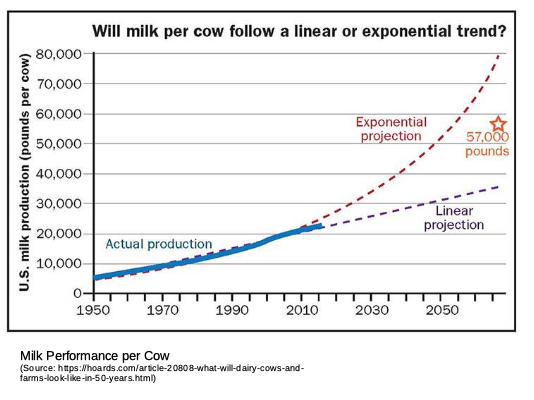
\includegraphics[width=7.42in,]{odg/milkcompperf} \caption{Yearly Milk Yield per Cow in the USA}\label{fig:milkcompperf}
\end{figure}

The Figure \ref{fig:moorelaw} below shows the development of computing power according to Moore's law.

\begin{figure}[!ht]
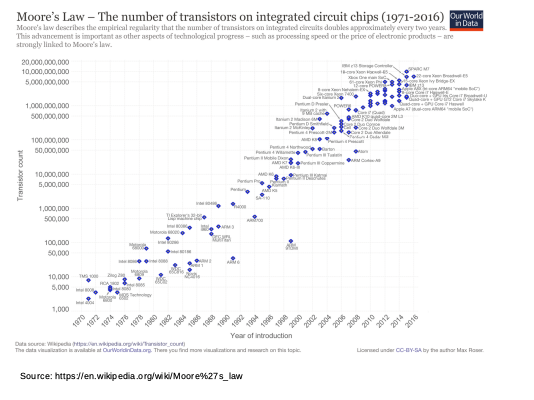
\includegraphics[width=7.42in,]{odg/moorelaw} \caption{Computing Performance According To Moore's Law}\label{fig:moorelaw}
\end{figure}

\hypertarget{quan-gen}{%
\chapter{Basics in Quantitative Genetics}\label{quan-gen}}

As already mentioned in section \ref{geno-pheno}, the central dogma of molecular biology tells us that the genotype is the basics of any phenotypic expression. The genotype of an individual is composed of a number of genes which are also called \textbf{loci}. In this section, we start with the simplest possible genetic architecture where the genotype is composed by just one locus. The connection between the genotype and the phenotype is modeled according to equation \eqref{eq:phengenenv}. The phenotype is assumed to be a quantitative trait. That means we are not looking at binary or categorical traits. Categorical traits can just take a limited number of different levels. Examples of categorical traits are the horn status in cattle or certain color characteristics. Quantitative traits do not take discrete levels but they show specific distributions.

\hypertarget{single-locus-quant-trait}{%
\section{Single Locus - Quantitative Trait}\label{single-locus-quant-trait}}

In Livestock there are not many examples where a quantitative trait is influenced by just one locus. But this case helps in understanding the foundation of more complex genetic architectures. We start by looking at the following idealized population (Figure \ref{fig:idealpopsingletrait}).

\begin{figure}[!ht]
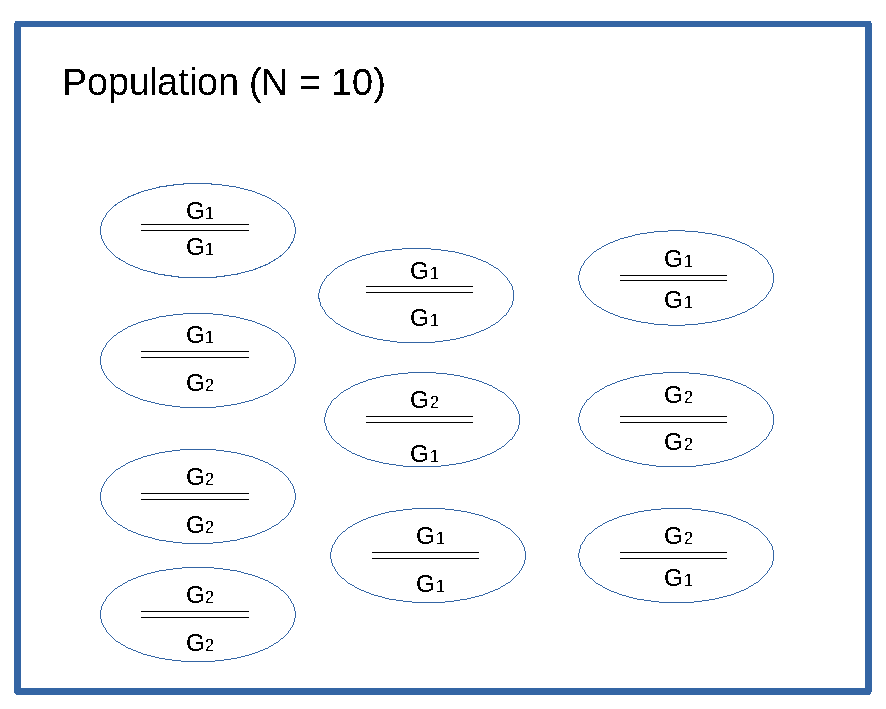
\includegraphics[width=1\linewidth,]{odg/idealpopsingletrait} \caption{Idealized Population With A Single Locus}\label{fig:idealpopsingletrait}
\end{figure}

\hypertarget{qg-terminology}{%
\subsection{Terminology}\label{qg-terminology}}

The different genetic variants that are present at our Locus \(G\) are called \textbf{alleles}. When looking at all individuals in the population for our locus, we have two different alleles \(G_1\) and \(G_2\). Hence, we call the locus \(G\) to be a \textbf{bi-allelic} locus. In any given individual of the population, the two alleles of the locus \(G\) together are called the individuals \textbf{genotype}. All possible combinations of the two alleles at the locus \(G\) leads to a total number of three genotypes. It is important to mention that the order of the alleles in a given genotype is not important. Hence, \(G_1G_2\) and \(G_2G_1\) are the same genotype. The two genotypes \(G_1G_1\) and \(G_2G_2\) are called \textbf{homozygous} and the genotype \(G_1G_2\) is called \textbf{heterozygous}.

\hypertarget{qg-frequency}{%
\section{Frequencies}\label{qg-frequency}}

To be able to characterize our population with respect to the locus of interest, we are first looking at some frequencies. These are measures of how often a certain allele or genotype does occur in our population. For our example population shown in Figure \ref{fig:idealpopsingletrait}, the \textbf{genotype frequencies} are

\begin{align}
f(G_1G_1) &= \frac{4}{10} = 0.4 \notag \\
f(G_1G_2) &= \frac{3}{10} = 0.3 \notag \\
f(G_2G_2) &= \frac{3}{10} = 0.3  \label{eq:genotypefreq}
\end{align}

The \textbf{allele frequencies} can be determined either by counting or they can be computed from the genotype frequencies.

\begin{align}
f(G_1) &= f(G_1G_1) + {1\over 2}*f(G_1G_2) = 0.55 \notag \\
f(G_2) &= f(G_2G_2) + {1\over 2}*f(G_1G_2) = 0.45 \label{eq:allelefreq}
\end{align}

\hypertarget{hw-eq}{%
\section{Hardy-Weinberg Equilibrium}\label{hw-eq}}

The Hardy-Weinberg equilibrium is the central law of how allele frequencies and genotype frequencies are related in an idealized population. Given the allele frequencies

\begin{align}
f(G_1) &= p \notag \\
f(G_2) &= q = 1-p
\label{eq:allelefreq}
\end{align}

During mating, we assume that in an idealized population alleles are combined independently. This leads to the genotype frequencies shown in Table \ref{tab:tabgenfreq}.

\begin{table}

\caption{\label{tab:tabgenfreq}Genotype Frequencies under Hardy-Weinberg equilibrium}
\centering
\begin{tabular}[t]{ccc}
\toprule
Alleles & $G_1$ & $G_2$\\
\midrule
$G_1$ & $f(G_1G_1) = p^2$ & $f(G_1G_2) = p*q$\\
$G_2$ & $f(G_1G_2) = p*q$ & $f(G_2G_2) = q^2$\\
\bottomrule
\end{tabular}
\end{table}

Summing up the heterozygous frequencies leads to

\begin{align}
f(G_1G_1) &= p^2 \notag \\
f(G_1G_2) &= 2pq \notag \\
f(G_2G_2) &= q^2
\label{eq:genofreq}
\end{align}

Comparing these expected genotype frequencies in a idealized population under the Hardy-Weinberg equilibrium to what we found for the small example population in Figure \ref{fig:idealpopsingletrait}, we can clearly say that the small example population is not in Hardy-Weinberg equilibrium.

\hypertarget{value-mean}{%
\section{Value and Mean}\label{value-mean}}

Our goal is still to improve our population at the genetic level. The term improvement implies the need for a quantitative assessment of our trait of interest. Furthermore, we have to be able to associate the genotypes in the population to the quantitative values of our trait.

\hypertarget{geno-value}{%
\subsection{Genotypic Values}\label{geno-value}}

The values \(V_{ij}\) to each genotype \(G_iG_j\) are assigned as shown in Figure \ref{fig:genotypicvalue}.

\begin{figure}[!ht]
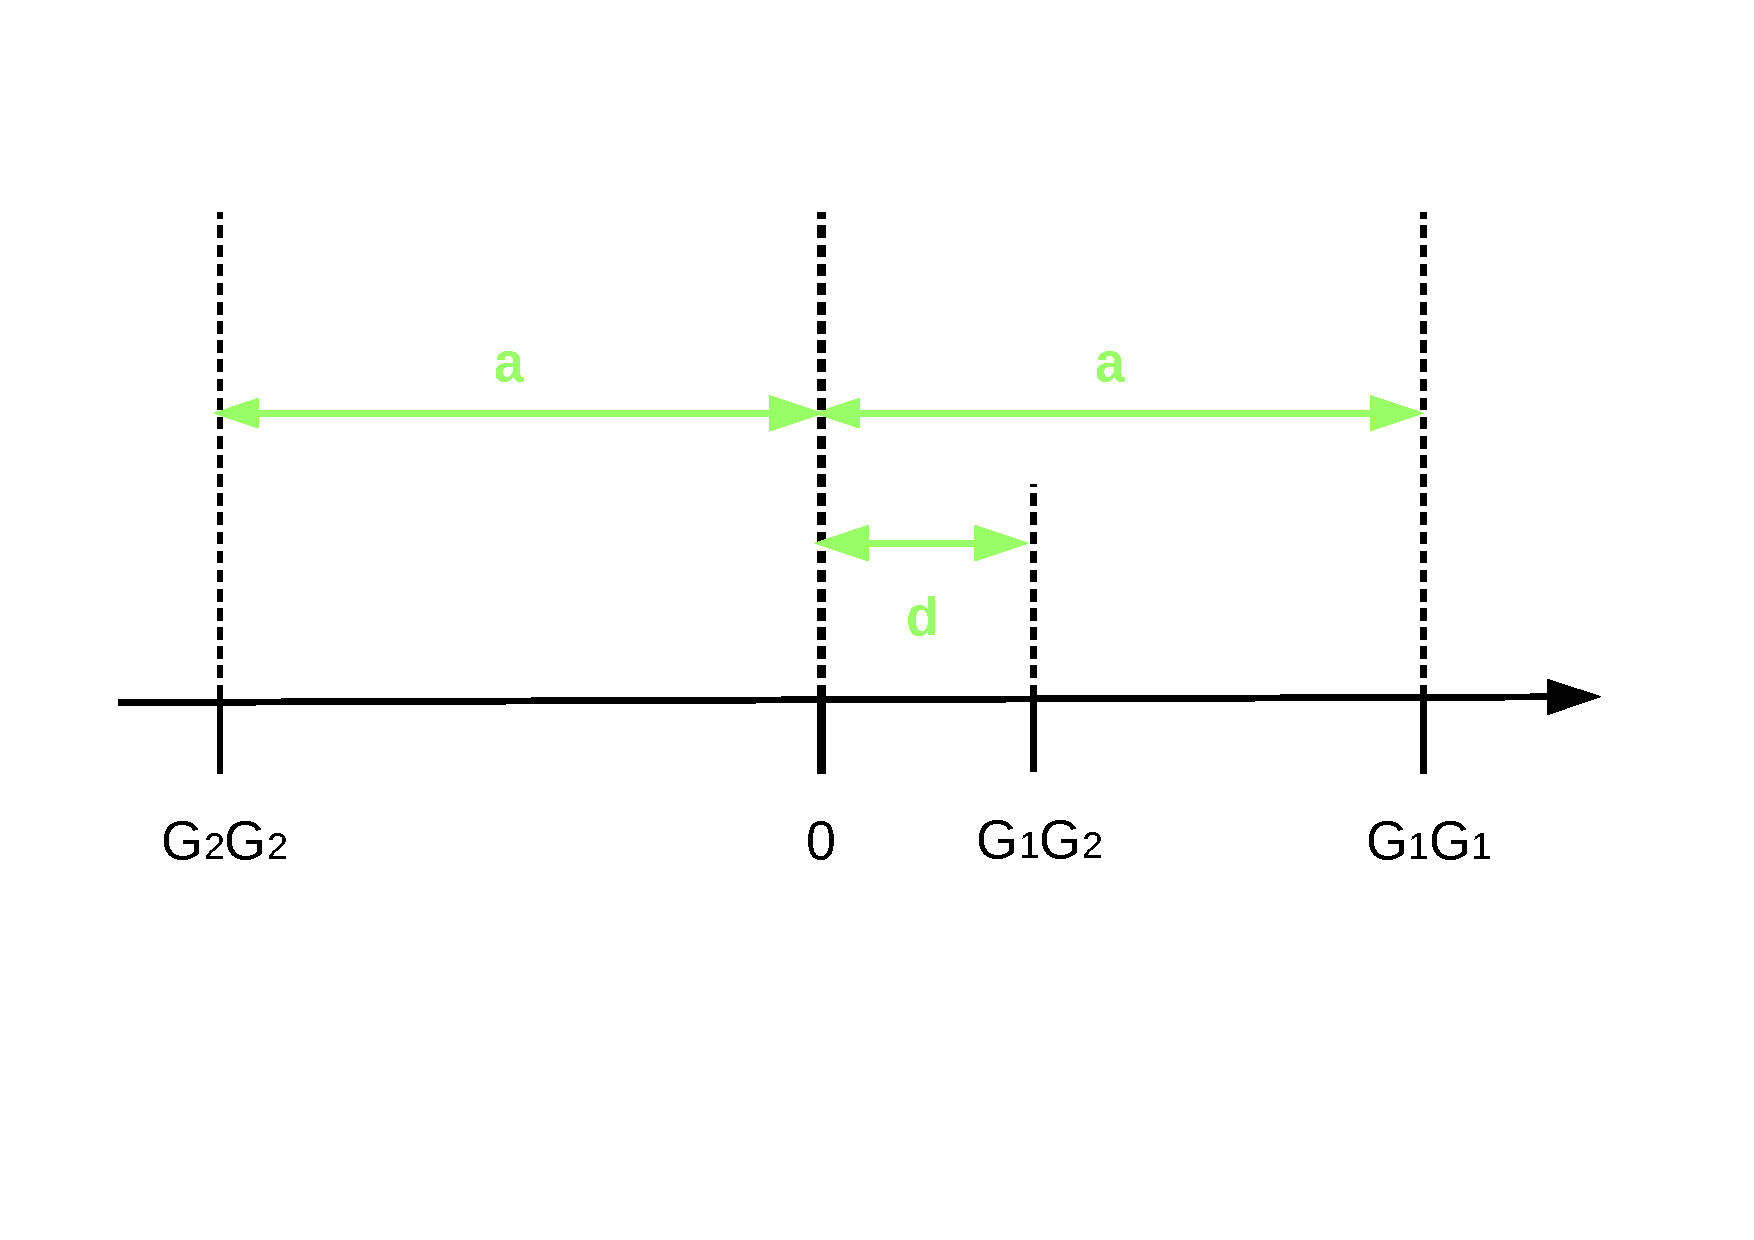
\includegraphics[width=1\linewidth,]{odg/genotypicvalue} \caption{Genotypic Values}\label{fig:genotypicvalue}
\end{figure}

The origin of the genotypic values is placed in the middle between the two homozygous genotypes \(G_2G_2\) and \(G_1G_1\). Here we are assuming that \(G_1\) is the favorable allele. This leads to values of \(+a\) for genotype \(G_1G_1\) and of \(-a\) for genotype \(G_2G_2\). The value of genotype \(G_1G_2\) is set to \(d\) and is called dominance deviation. Table \ref{tab:tabsumgenvalue} summarizes the values for all genotypes.

\begin{table}

\caption{\label{tab:tabsumgenvalue}Values for all Genotypes}
\centering
\begin{tabular}[t]{ccc}
\toprule
Variable & Genotype & Values\\
\midrule
$V_{11}$ & $G_1G_1$ & a\\
$V_{12}$ & $G_1G_2$ & d\\
$V_{22}$ & $G_2G_2$ & -a\\
\bottomrule
\end{tabular}
\end{table}

\hypertarget{pop-mean}{%
\subsection{Population Mean}\label{pop-mean}}

For the complete population, we can compute the \textbf{population mean} (\(\mu\)) of all values at the locus \(G\). This mean corresponds to the expected value and is computed as

\begin{align}
\mu &= V_{11} * f(G_1G_1) + V_{12} * f(G_1G_2) + V_{22} * f(G_2G_2) \notag \\
    &= a * p^2 + d *2pq + (-a) * q^2 \notag \\
    &= (p-q)a + 2pqd
\label{eq:popmean}
\end{align}

The population mean depends on the values \(a\) and \(d\) and on the allele frequencies \(p\) and \(q\). The larger the difference between \(p\) and \(q\) the more influence the value \(a\) has in \(\mu\), because for very different \(p\) and \(q\) the product \(2pq\) is very small. On the other hand, if \(p=q=0.5\), then \(\mu = 0.5d\). For loci with \(d=0\), the population mean \(\mu = (p-q)a\) and hence, if in addition we have \(p=q\), then \(\mu=0\).

\hypertarget{breed-value}{%
\subsection{Breeding Values}\label{breed-value}}

The term \textbf{breeding value} is defined as shown in Definition \ref{def:defbreedingvalue}.

\begin{definition}[Breeding Value]
\protect\hypertarget{def:defbreedingvalue}{}{\label{def:defbreedingvalue} \iffalse (Breeding Value) \fi{} }The breeding value of an animal \(i\) is defined as two times the difference between the mean value of offsprings of animal \(i\) and the population mean.
\end{definition}

Applying this definition and using the parameters that we have computed so far leads to the following formulas for the breeding value of an animal with a certain genotype.

\hypertarget{breeding-value-for-g_1g_1}{%
\subsubsection{\texorpdfstring{Breeding value for \(G_1G_1\)}{Breeding value for G\_1G\_1}}\label{breeding-value-for-g_1g_1}}

Assume that we have a given parent \(S\) with a genotype \(G_1G_1\) and we want to compute its breeding value. Let us further suppose that our single parent \(S\) is mated to a potentially infinite number of animals from the idealized population, then we can deduce the following mean genotypic value for the offspring of parent \(S\).

\vspace{5ex}

\begin{center}
\begin{tabular}{|c|c|c|}
\hline
& \multicolumn{2}{|c|}{Mates of $S$} \\
\hline
& $f(G_1) = p$       &  $f(G_2) = q$   \\
\hline
Parent $S$       &                    &                 \\
\hline
$f(G_1) = 1$ &  $f(G_1G_1) = p$   &  $f(G_1G_2) = q$\\
\hline
\end{tabular}
\end{center}

\vspace{5ex}

Because parent \(S\) has genotype \(G_1G_1\), the frequency \(f(G_1)\) of a \(G_1\) allele coming from \(S\) is \(1\) and the frequency \(f(G_2)\) of a \(G_2\) allele is 0. The expected genetic value (\(\mu_{11}\)) of the offspring of animal \(S\) can be computed as

\begin{equation}
\mu_{11} = p*a + q*d
\label{eq:MeanOffGen11}
\end{equation}

Applying definition \ref{def:defbreedingvalue}, we can compute the breeding value (\(BV_{11}\)) for animal \(S\) as shown in equation \eqref{eq:BVGen11} while using the results given by equations \eqref{eq:MeanOffGen11} and \eqref{eq:popmean}.

\begin{align}
BV_{11} &=  2*(\mu_{11} - \mu)  \notag \\
        &=  2\left(pa + qd - \left[(p - q)a + 2pqd \right] \right) \notag\\
        &=  2\left(pa + qd - (p - q)a - 2pqd \right) \notag\\
        &=  2\left(qd + qa - 2pqd\right) \notag \\
        &=  2\left(qa + qd(1 - 2p)\right) \notag \\
        &=  2q\left(a + d(1 - 2p)\right) \notag \\
        &=  2q\left(a + (q-p)d\right)
\label{eq:BVGen11}
\end{align}

Breeding values for parents with genotypes \(G_2G_2\) and \(G_1G_2\) are derived analogously.

\hypertarget{breeding-value-for-g_2g_2}{%
\subsubsection{\texorpdfstring{Breeding value for \(G_2G_2\)}{Breeding value for G\_2G\_2}}\label{breeding-value-for-g_2g_2}}

First, we determine the expected genotypic value for offsprings of a parent \(S\) with genotype \(G_2G_2\)

\vspace{5ex}

\begin{center}
\begin{tabular}{|c|c|c|}
\hline
& \multicolumn{2}{|c|}{Mates of parent $S$} \\
\hline
& $f(G_1) = p$       &  $f(G_2) = q$   \\
\hline
Parent $S$       &                    &                 \\
\hline
$f(G_2) = 1$ &  $f(G_1G_2) = p$   &  $f(G_2G_2) = q$\\
\hline
\end{tabular}
\end{center}

\vspace{5ex}

The expected genetic value (\(\mu_{22}\)) of the offspring of animal \(S\) can be computed as

\begin{equation}
\mu_{22} = pd - qa
\label{eq:MeanOffGen22}
\end{equation}

The breeding value \(BV_{22}\) corresponds to

\begin{align}
BV_{22} &=   2*(\mu_{22} - \mu)  \notag \\
        &=   2\left(pd - qa - \left[(p - q)a + 2pqd \right] \right) \notag \\
        &=   2\left(pd - qa - (p - q)a - 2pqd \right) \notag \\
        &=   2\left(pd - pa - 2pqd\right) \notag \\
        &=   2\left(-pa + p(1-2q)d\right) \notag \\
        &=  -2p\left(a + (q - p)d\right)
\label{eq:BVGen22}
\end{align}

\hypertarget{breeding-value-for-g_1g_2}{%
\subsubsection{\texorpdfstring{Breeding value for \(G_1G_2\)}{Breeding value for G\_1G\_2}}\label{breeding-value-for-g_1g_2}}

The genotype frequencies of the offsprings of a parent \(S\) with a genotype \(G_1G_2\) is determined in the following table.

\vspace{5ex}

\begin{center}
\begin{tabular}{|c|c|c|}
\hline
& \multicolumn{2}{|c|}{Mates of parent $S$} \\
\hline
& $f(G_1) = p$       &  $f(G_2) = q$   \\
\hline
Parent $S$       &                    &                 \\
\hline
$f(G_1) = 0.5$ &  $f(G_1G_1) = 0.5p$   &  $f(G_1G_2) = 0.5q$\\
\hline
$f(G_2) = 0.5$ &  $f(G_1G_2) = 0.5p$   &  $f(G_2G_2) = 0.5q$\\
\hline
\end{tabular}
\end{center}

\vspace{5ex}

The expected mean genotypic value of the offsprings of parent \(S\) with genotype \(G_1G_2\) is computed as

\begin{equation}
\mu_{12} = 0.5pa + 0.5d - 0.5qa = 0.5\left[(p-q)a + d \right]
\label{eq:MeanOffGen12}
\end{equation}

The breeding value \(BV_{12}\) corresponds to

\begin{align}
ZW_{12} &=   2*(\mu_{12} - \mu) \notag \\
        &=   2\left(0.5(p-q)a + 0.5d - \left[(p - q)a + 2pqd \right] \right) \notag \\
        &=   2\left(0.5pa - 0.5qa + 0.5d - pa + qa - 2pqd \right) \notag \\
        &=   2\left(0.5(q-p)a + (0.5 - 2pq)d \right) \notag \\
        &=   (q-p)a + (1-4pq)d  \notag \\
        &=   (q-p)a + (p^2 + 2pq + q^2 -4pq)d  \notag \\
        &=   (q-p)a + (p^2 - 2pq + q^2)d  \notag \\
        &=   (q-p)a + (q - p)^2d   \notag \\
        &=   (q-p)\left[a + (q-p)d \right]
\label{eq:BVGen12}
\end{align}

\hypertarget{summary-of-breeding-values}{%
\subsubsection{Summary of Breeding Values}\label{summary-of-breeding-values}}

The term \(a + (q-p)d\) appears in all three breeding values. We replace this term by \(\alpha\) and summarize the results in the following table.

\vspace{5ex}

\begin{center} 
\begin{tabular}{|c|c|}
  \hline
  Genotype  &  Breeding Value\\
  \hline
  $G_1G_1$  &  $2q\alpha$    \\
  \hline
  $G_1G_2$  &  $(q-p)\alpha$ \\
  \hline
  $G_2G_2$  &  $-2p\alpha$   \\
  \hline
\end{tabular}
\end{center}

\vspace{5ex}

\hypertarget{allele-substitution}{%
\subsection{Allele Substitution}\label{allele-substitution}}

Comparing the genotype \(G_2G_2\) with the genotype \(G_1G2\), one of the differences is in the number of \(G_1\)-alleles. \(G_2G_2\) has zero \(G_1\)-alleles and \(G_1G_2\) has one \(G_1\)-allele.

Let us imagine that we take animal \(i\) with a \(G_2G_2\) genotype and use the CRISPR-CAS genome editing technology to replace one of the \(G_2\) alleles in animal \(i\) by a \(G_1\) allele (see Figure \ref{fig:genome-editing-allele-substitution}). After applying the gene editing procedure to animal \(i\) at locus \(G\), animal \(i\) would have genotype \(G_1G_2\).

\begin{figure}[!ht]
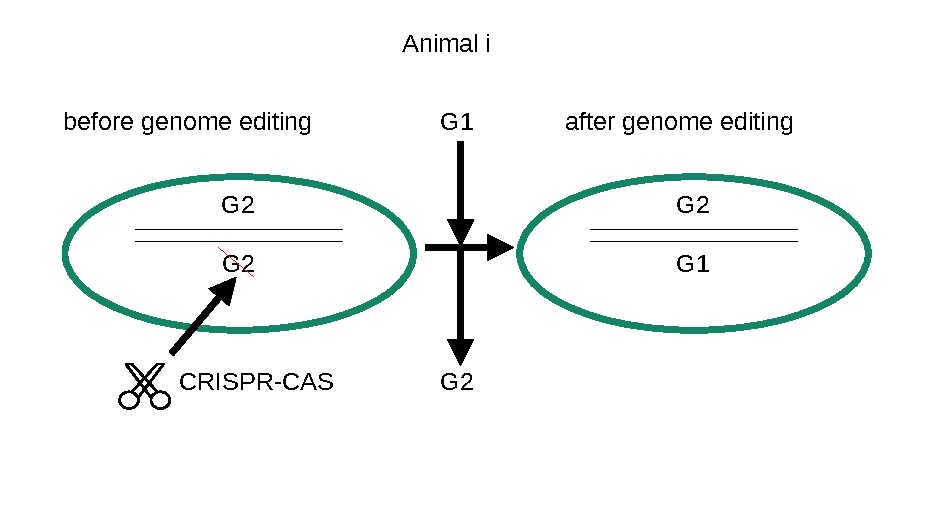
\includegraphics[width=1\linewidth,]{odg/genome-editing-allele-substitution} \caption{Schematic Depiction of Genome Editing on Animal i}\label{fig:genome-editing-allele-substitution}
\end{figure}

Due to the application of genome editing at locus \(G\) of animal \(i\) the breeding value changed. Before the genome editing procedure it was \(BV_{22}\) and after genome editing the breeding value of animal \(i\) corresponds to \(BV_{12}\). So the effect of replacing a \(G_2\) allele by a \(G_1\) allele on the breeding value corresponds to the difference \(BV_{12} - BV_{22}\). The computation of this difference between the breeding value \(BV_{12}\) and \(B_{22}\) results in

\begin{align}
    BV{12} - BV_{22} &=   (q-p)\alpha - \left( -2p\alpha \right)  \notag \\
                      &=   (q-p)\alpha + 2p\alpha \notag \\
                      &=   (q-p+2p)\alpha \notag \\
                      &=   (q+p)\alpha \notag \\
                      &=   \alpha
  \label{eq:AdditiveBv1}
\end{align}

The analogous computation can be done by comparing the breeding values \(BV_{11}\) and \(BV_{12}\).

\begin{align}
    BV_{11} - BV_{12} & = & 2q\alpha - (q-p)\alpha \notag \\
                      & = & \left(2q - (q-p)\right)\alpha \notag\\
                      & = & \alpha 
  \label{eq:AdditiveBv2}
\end{align}

Because the differences between breeding values computed in \eqref{eq:AdditiveBv1} and \eqref{eq:AdditiveBv2} are equal, we can conclude that the breeding values show a linear dependence on the number of \(G_1\) alleles. This is the reason why the breeding values are also called additive effects, because adding a further \(G_1\) allele instead of a \(G_2\) allel has always the same effect on the breeding values, namely just adding the constant allele substitution effect \(\alpha\).

\hypertarget{dominance-deviation}{%
\subsection{Dominance Deviation}\label{dominance-deviation}}

When looking at the difference between the genotypic value \(V_{ij}\) and the breeding value \(BV_{ij}\) for each of the three genotypes, we get the following results.

\begin{align}
  V_{11} - BV_{11} &=   a - 2q \alpha \notag \\
                   &=   a - 2q \left[ a + (q-p)d \right] \notag \\
                   &=   a - 2qa -2q(q-p)d \notag \\
                   &=   a(1-2q) - 2q^2d + 2pqd \notag \\
                   &=   \left[(p - q)a + 2pqd\right] - 2q^2d \notag \\
                   &=   \mu + D_{11} 
  \end{align}

\begin{align}
  V_{12} - BV{12} &=   d - (q-p)\alpha \notag \\
                   &=   d - (q-p)\left[ a + (q-p)d \right] \notag \\
                   &=   \left[(p-q)a + 2pqd\right] + 2pqd \notag \\
                   &=   \mu + D_{12}
  \end{align}

\begin{align}
  V_{22} - BV_{22} &=   -a - (-2p\alpha) \notag \\
                   &=   -a + 2p\left[ a + (q-p)d \right] \notag \\
                   &=   \left[(p-q)a + 2pqd\right] - 2p^2d \notag \\
                   &=   \mu + D_{22} \notag
  \end{align}

The difference all contain the population mean \(\mu\) plus a certain deviation. This deviation term is called \textbf{dominance deviation}.

\hypertarget{summary-of-values}{%
\subsection{Summary of Values}\label{summary-of-values}}

The following table summarizes all genotypic values all breeding values and the dominance deviations.

\vspace{5ex}

\begin{center} 
\begin{tabular}{|c|c|c|c|}
   \hline
   Genotyp  &  genotypic value     &  Breeding Value    &  Dominance Deviation \\
   $G_iG_j$ &  $V_{ij}$            &  $BV_{ij}$         &  $D_{ij}$           \\
   \hline
   $G_1G_1$ &  $a$                 &  $2q\alpha$        &  $-2q^2d$          \\
   \hline
   $G_1G_2$ &  $d$                 &  $(q-p)\alpha$     & $2pqd$             \\
   \hline
   $G_2G_2$ &  $-a$                &  $-2p\alpha$       & $-2p^2d$           \\
   \hline
\end{tabular}
\end{center}

\vspace{5ex}

The formulas in the above shown table assume that \(G_1\) is the favorable allele with frequency \(f(G_1) = p\). The allele frequency of \(G_2\) is \(f(G_2) = q\). Since we have a bi-allelic locus \(p+q=1\).

Based on the definition of dominance deviation, the genotypic values \(V_{ij}\) can be decomposed into the components population mean (\(\mu\)), breeding value (\(BV_{ij}\)) and dominance deviation (\(D_{ij}\)) according to equation \eqref{eq:SeparationGenoValue}.

\begin{align}
V_{ij} &=   \mu + BV_{ij} + D_{ij}
\label{eq:SeparationGenoValue}
\end{align}

Taking expected values on both sides of equation \eqref{eq:SeparationGenoValue} and knowing that the population mean \(\mu\) was defined as the expected value of the genotypic values in the population, i.e.~\(E\left[ V \right] = \mu\), it follows that the expected values of both the breeding values and the dominance deviations must be \(0\). More formally, we have

\begin{align}
E\left[ V \right] &=  E\left[ \mu + BV + D \right] \notag \\
                  &=  E\left[ \mu \right]  + E\left[ BV \right] + E\left[ D \right] \notag \\
                  &=  \mu
\label{eq:ExpValueGenBvDom}
\end{align}

From the last line in equation \eqref{eq:ExpValueGenBvDom}, it follows that \(E\left[ BV \right] = E\left[ D \right] = 0\). This also shows that both breeding values and dominance deviations are defined as deviation from a given mean.

\hypertarget{variances}{%
\section{Variances}\label{variances}}

The population mean \(\mu\) and derived from that the breeding values were defined as expected values. Their main purpose is to assess the state of a given population with respect to a certain genetic locus and its effect on a phenotypic trait of interest. One of our primary goals in livestock breeding is to improve the populations at the genetic level through the means of selection and mating. Selection of potential parents that produce offspring that are closer to our breeding goals is only possible, if the selection candidates show a certain level of variation in the traits that we are interested in. In populations where there is no variation which means that all individuals are exactly at the same level, it is not possible to select potential parents for the next generation.

In statistics the measure that is most often used to assess variation in a certain population is called \textbf{variance}. For any given discrete random variable \(X\) the variance is defined as the second central moment of \(X\) which is computed as shown in equation \eqref{eq:VarianceDiscreteRV}.

\begin{equation}
Var\left[X\right] = \sum_{x_i \in \mathcal{X}} (x_i - \mu_X)^2 * f(x_i)
\label{eq:VarianceDiscreteRV}
\end{equation}

\vspace*{1ex}

\begin{tabular}{p{1cm}p{1cm}p{6cm}}
  where & $\mathcal{X}$: &  set of all possible $x$-values\\
        & $f(x_i)$       &  probability that $x$ assumes the value of $x_i$ \\
        & $\mu_X $       &  expected value $E\left[X\right]$ of $X$
  \end{tabular}

\vspace*{2ex}

In this section we will be focusing on separating the obtained variances into different components according to their causative sources. Applying the definition of variance given in equation \eqref{eq:VarianceDiscreteRV} to the genotypic values \(V_{ij}\), we obtain the following expression.

\begin{align}
\sigma_G^2 = Var\left[V\right] &=   (V_{11} - \mu)^2 * f(G_1G_1) \notag \\
                               &  +\  (V_{12} - \mu)^2 * f(G_1G_2) \notag \\
                               &  +\  (V_{22} - \mu)^2 * f(G_2G_2)
\label{eq:VarianceGenotypicValue}
\end{align}

where \(\mu = (p - q)a + 2pqd\) the population mean.

Based on the decomposition of the genotypic value \(V_{ij}\) given in \eqref{eq:SeparationGenoValue}, the difference between \(V_{ij}\) and \(\mu\) can be written as the sum of the breeding value and the dominance deviation. Then \(\sigma_G^2\) can be written as

\begin{align}
\sigma_G^2 = Var\left[V\right] &=   (BV_{11} + D_{11})^2 * f(G_1G_1) \notag \\
                               &  +\  (BV_{12} + D_{12})^2 * f(G_1G_2) \notag \\
                               &  +\  (BV_{22} + D_{22})^2 * f(G_2G_2)
\label{eq:GeneticVarianceBVDom}
\end{align}

Inserting the expressions for the breeding values \(BV_{ij}\) and for the dominance deviation \(D_{ij}\) found earlier and simplifying the equation leads to the result in \eqref{eq:FinalGeneticVariance}. A more detailed derivation of \(\sigma_G^2\) is given in the appendix (\ref{appendix-derivations}) of this chapter.

\begin{align}
  \sigma_G^2 &=  2pq\alpha^2 + \left(2pqd \right)^2 \notag\\
             &=  \sigma_A^2 + \sigma_D^2
\label{eq:FinalGeneticVariance}             
\end{align}

The formula in equation \eqref{eq:FinalGeneticVariance} shows that \(\sigma_G^2\) consists of two components. The first component \(\sigma_A^2\) is called the \textbf{genetic additive variance} and the second component \(\sigma_D^2\) is termed \textbf{dominance variance}. As shown in equation \eqref{eq:VarBV} \(\sigma_A^2\) corresponds to the variance of the breeding values. Because we have already seen that the breeding values are additive in the number of favorable alleles, \(\sigma_A^2\) is called genetic additive variance. Because \(\sigma_D^2\) corresponds to the variance of the dominance deviation effects (see equation \eqref{eq:VarDom}) it is called dominance variance.

\hypertarget{extension-to-more-loci}{%
\section{Extension To More Loci}\label{extension-to-more-loci}}

When only a single locus is considered, the genotypic values (\(V_{ij}\)) can be decomposed according to equation \eqref{eq:SeparationGenoValue} into population mean, breeding value and dominance deviation. When a genotype refers to more than one locus, the genotypic value may contain an additional deviation caused by non-additive combination effects.

\hypertarget{epistatic-interaction}{%
\subsection{Epistatic Interaction}\label{epistatic-interaction}}

Let \(V_A\) be the genotypic value of locus \(A\) and \(V_B\) denote the genotypic value of a second locus \(B\), then the total genotypic value \(V\) attributed to both loci \(A\) and \(B\) can be written as

\begin{align}
V &= V_A + V_B + I_{AB} 
\label{eq:AggregateGenotypicValueTwoLoci}
\end{align}

where \(I_{AB}\) is the deviation from additive combination of these genotypic values. When computing the population mean earlier in this chapter, we assumed that \(I\) was zero for all combinations of genotypes. If \(I\) is not zero for any combination of genes at different loci, those genes are said to \textbf{interact} with each other or to exhibit \textbf{epistasis}. The deviation \(I\) is called interaction deviation or epistatic deviation. If \(I\) is zero, the genes are called to act additively between loci. Hence \emph{additive action} may mean different things. When referring to one locus, it means absence of dominance. When referring to different loci, it means absence of epistasis.

Interaction between loci may occur between pairs or between higher numbers of different loci. The complex nature of higher order interactions, i.e., interactions between higher number of loci does not need to concern us. Because in the total genotypic value \(V\), interaction deviations of all sorts are treated together in an overall interaction deviation \(I\).

Applying the decomposition of the genotypic values \(V_A\) of locus \(A\) and \(V_B\) of locus \(B\) as shown in \eqref{eq:SeparationGenoValue} leads to

\begin{align}
V &= V_A + V_B + I_{AB} \notag \\
  &= \mu_A + BV_A + D_A + \mu_B + BV_B + D_B + I_{AB}
\label{eq:DecomposeGenotypicValueTwoLoci}
\end{align}

Collecting terms in \eqref{eq:DecomposeGenotypicValueTwoLoci} as follows

\begin{align}
\mu &= \mu_A + \mu_B \notag \\
U   &= BV_A + BV_B \notag \\
D   &= D_A + D_B \notag \\
I   &= I{AB}
\label{eq:CollectVariables}
\end{align}

The decomposition shown in \eqref{eq:DecomposeGenotypicValueTwoLoci} and the collection of variables (see \eqref{eq:CollectVariables}) can be generalized to more than two loci. This leads to the following generalized form of decomposing the overall total genotype \(V\) for the case of multiple loci affecting a certain trait of interest.

\begin{equation}
V = \mu + U + D + I
\label{eq:AggregateGenotypicValueMultipleLoci}
\end{equation}

where \(U\) is the sum of the breeding values attributable to the separate loci and \(D\) is the sum of all dominance deviations. For our purposes in livestock breeding where we want to assess the genetic potential of a selection candidate to be a parent of offspring forming the next generation, the \textbf{breeding value} is the most important quantity. The breeding value is of primary importance because a given parent passes a random sample of its alleles to its offspring. We have seen in section \ref{allele-substitution} that breeding values are additive in the number of favorable alleles. Hence the more favorable alleles a given parent passes to its offspring the higher the breeding value of this parent.

On the other hand, the dominance deviation measures the effect of a certain genotype occurring in an individual and the interaction deviation estimates the effects of combining different genotypes at different loci in the genome. But because parents do not pass complete genotypes nor do they pass stretches of DNA with several loci, but only a random collection of its alleles, it is really the breeding value that is of primary importance in assessing the genetic potential of a given selection candidate.

\hypertarget{interaction-variance}{%
\subsection{Interaction Variance}\label{interaction-variance}}

If genotypes at different loci show epistatic interaction effects as described in section \ref{epistatic-interaction}, the interactions give rise to an additional variance component called \(V_I\), which is the variance of interaction deviations. This new variance component \(V_I\) can be further decomposed into sub-components. The first level of sub-components is according to the number of loci that are considered. Two-way interactions involve two loci, three-way interactions consider three loci and in general \(n\)-way interactions arise from \(n\) different loci. The next level of subdivision is according to whether they include additive effects, dominance deviations or both.

In general it can be said that for practical purposes, interaction effects explain only a very small amount of the overall variation. As already mentioned in section @ref(\#epistatic-interaction) for livestock breeding, we are mostly interested in the additive effects. This is also true when looking at the variance components. Hence dominance variance and variances of interaction deviations are not used very often in practical livestock breeding application.

\hypertarget{genetic-models}{%
\section{Genetic Models}\label{genetic-models}}

In this chapter, we have seen how to model the genetic basis of a quantitative trait when a single locus affects the trait of interest. We call this a single-locus model. When several loci have an effect on a certain trait, then we talk about a \textbf{polygenic model}. Letting the number of loci affecting a certain phenotype tend to infinity, the resulting model is called \textbf{infinitesimal model}.

From a statistical point of view, the breeding values in an infinitesimal model are considered as a random effect with a known distribution. Due to the central limit theorem, this distribution is assumed to be a normal distribution. The central limit theorem says that the distribution of any sum of a large number of very small effects converges to a normal distribution. For our case where a given trait of interest is thought to be influenced by a large number of genetic loci each having a small effect, the sum of the breeding values of all loci together can be approximated by a normal distribution. Figure (\ref{fig:hist-clt}) shows the distribution for a sum of 10, 100 and 1000 components each. The histograms show a better approximation to the normal distribution the larger the number of components considered in the sum.

\begin{figure}[!ht]
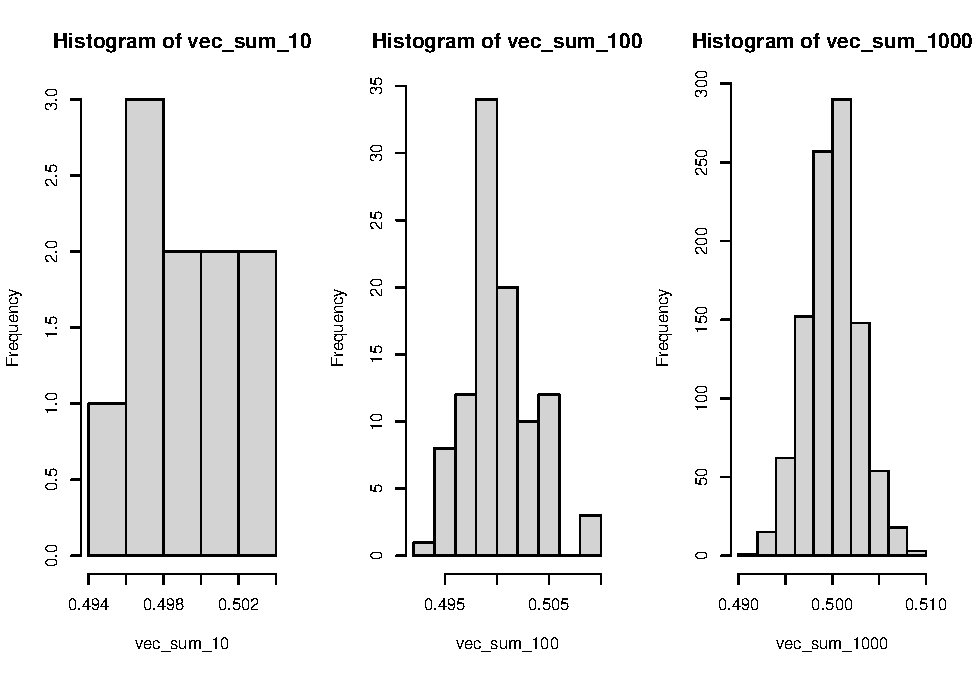
\includegraphics{lbgfs2021-cn_files/figure-latex/hist-clt-1} \caption{Distribution of Sums of Different Numbers of Components}\label{fig:hist-clt}
\end{figure}

\hypertarget{model-usage-in-routine-evaluations}{%
\subsection{Model Usage In Routine Evaluations}\label{model-usage-in-routine-evaluations}}

Traditional prediction of breeding values before the introduction of genomic selection is based on the infinitesimal model. When genomic selection was introduced which takes into account the information from a large number of loci, genomic breeding values are estimated using a polygenic model.

\hypertarget{appendix-derivations}{%
\section{Appendix: Derivations}\label{appendix-derivations}}

This section shows how the genetic variance in equation \eqref{eq:FinalGeneticVariance} is computed.

\begin{align}
\sigma_G^2  &=   (BV_{11} + D_{11})^2 * p^2                                       \notag \\
            &   +\  (BV_{12} + D_{12})^2 * 2pq                                    \notag \\
            &   +\  (BV_{22} + D_{22})^2 * q^2                                    \notag \\
            &=      \left(2q\alpha - 2q^2d   \right)^2 * p^2                      \notag \\
            &   +\  \left((q-p)\alpha + 2pqd \right)^2 * 2pq                      \notag \\
            &   +\  \left(-2p\alpha - 2p^2d  \right)^2 * q^2                      \notag \\
            &=      \left(4q^2\alpha^2 - 8q^3d\alpha + 4q^4d^2  \right) * p^2     \notag \\
            &   +\  \left(q^2\alpha^2 - 2pq\alpha^2 + p^2\alpha^2
                           - 4(q-p)pqd\alpha + 4p^2q^2d^2\right) * 2pq            \notag \\
            &   +\  \left(4p^2\alpha^2 + 8p^3d\alpha + 4p^4\alpha^2 \right) * q^2 \notag \\
            &=      4p^2q^2\alpha^2 - 8p^2q^3d\alpha + 4p^2q^4d^2                 \notag \\
            &   +\  2pq^3\alpha^2 - 4p^2q^2\alpha^2+ 2p^3q\alpha^2                \notag \\
            &   -\  8p^3q^2d\alpha + 8p^2q^3d\alpha + 8p^3q^3d^2                  \notag \\
            &   +\  4p^2q^2\alpha^2 + 8p^3q^2d\alpha + 4p^4q^2d^2                 \notag \\
            &=      4p^2q^2\alpha^2 + 4p^2q^4d^2                                  \notag \\
            &   +\  2pq^3\alpha^2 + 2p^3q\alpha^2                                 \notag \\
            &   +\  8p^3q^3d^2                                                    \notag \\
            &   +\  4p^4q^2d^2                                                    \notag \\
            &=      2pq\alpha^2 \left(p^2 + 2pq + q^2 \right)                     \notag \\
            &   +\  \left(2pqd \right)^2 \left(p^2 + 2pq + q^2 \right)            \notag \\
            &=      2pq\alpha^2 + \left(2pqd \right)^2                            \notag \\
            &=      \sigma_A^2 + \sigma_D^2
\label{eq:GenVarZWD}
\end{align}

From the last two lines of \eqref{eq:GenVarZWD} it follows that \(\sigma_A^2 = 2pq\alpha^2\) and \(\sigma_D^2 = \left(2pqd \right)^2\). It can be shown that \(\sigma_A^2\) corresponds to the squared breeding values times the associated genotype frequencies. Because the expected values of the breeding values is zero, \(\sigma_A^2\) is equivalent to the variance of the breeding values.

\begin{align}
\sigma_A^2 &= Var\left[ BV \right] = (BV_{11} - E\left[ BV \right])^2 * f(G_1G_1)  \notag \\
           &   + (BV_{12} - E\left[ BV \right])^2 * f(G_1G_2)  \notag \\
           &   + (BV_{22} - E\left[ BV \right])^2 * f(G_2G_2) \notag \\
           &= BV_{11}^2 * f(G_1G_1) + BV_{12}^2 * f(G_1G_2) + BV_{22}^2 * f(G_2G_2) \notag \\
           &= \left(2q \alpha \right)^2 * p^2 +  \left((q-p) \alpha \right)^2 * 2pq + \left(-2p \alpha \right)^2 * q^2 \notag \\
           &= 4p^2 q^2 \alpha^2 + \left(q^2 \alpha^2 -2pq\alpha^2 + p^2 \alpha^2 \right) * 2pq + 4p^2q^2\alpha^2 \notag \\
           &= 8p^2 q^2 \alpha^2 + 2pq^3\alpha^2 -4p^2q^2\alpha^2 + 2p^3q\alpha^2 \notag \\
           &= 4p^2 q^2 \alpha^2 + 2pq^3\alpha^2  + 2p^3q\alpha^2 \notag \\
           &= 2pq\alpha^2 \left(2pq + q^2 + p^2 \right) \notag \\
           &= 2pq\alpha^2
\label{eq:VarBV}
\end{align}

In the above derivation in \eqref{eq:VarBV} of the variance of the breeding values, we were using the fact that the expected value \(E\left[ BV \right]=0\). This can be shown more formally as follows

\begin{align}
E\left[ BV \right]  &=  BV_{11} * f(G_1G_1) + BV_{12} * f(G_1G_2)  + BV_{22} * f(G_2G_2) \notag \\
                    &=  2q \alpha * p^2 + (q-p) \alpha * 2pq + (-2p \alpha) * q^2 \notag \\
                    &=  2p^2q \alpha + 2pq^2 \alpha - 2p^2q\alpha - 2pq^2\alpha \notag \\
                    &=  0
\label{eq:ExpectedValueBV}
\end{align}

Similarly to \eqref{eq:VarBV} we can show that \(\sigma_D^2\) corresponds to the squared dominance deviations times the frequencies of the corresponding genotypes. That is the reason why \(\sigma_D^2\) is called dominance variance.

\begin{align}
\sigma_D^2  &=  D_{11}^2 * f(G_1G_1) + D_{12}^2 * f(G_1G_2) + D_{22}^2 * f(G_2G_2) \notag \\
            &=   (- 2q^2d)^2 * p^2 + (2pqd)^2 * 2pq + (- 2p^2d)^2 * q^2 \notag \\
            &=  4p^2q^4d^2 + 8p^3q^3d^2 + 4p^4q^2d^2 \notag \\
            &=  4p^2q^2d^2 \left( q^2 + 2pq + p^2 \right) \notag \\
            &=  4p^2q^2d^2 
\label{eq:VarDom}
\end{align}

\cleardoublepage

\hypertarget{appendix-appendix}{%
\appendix}


\hypertarget{intro-linalg}{%
\chapter{Introduction To Linear Algebra}\label{intro-linalg}}

Linear Algebra is a large area. A short overview can be seen in a video (\url{https://youtu.be/kjBOesZCoqc}) by \citep{3Blue1Brown2016}. In this course we only need the following three topics from the large field of linear algebra.

\begin{enumerate}
\def\labelenumi{\arabic{enumi}.}
\tightlist
\item
  Vectors
\item
  Matrices and
\item
  Systems of linear equations.
\end{enumerate}

\hypertarget{intro-linalg-glimpse-ahead}{%
\section{Glimpse Ahead}\label{intro-linalg-glimpse-ahead}}

The central topic of this course is the prediction of breeding values. Most approaches to predict breeding values require the solution of large systems of linear equations. These systems of equations are written down using vectors and matrices. Hence the three mentioned topics are important to understand at a level that they can be used as tools for the prediction of breeding values.

\hypertarget{intro-linalg-vectors}{%
\section{Vectors}\label{intro-linalg-vectors}}

The material of this section is largely based on the video tutorial (\url{https://youtu.be/fNk_zzaMoSs}) from \citep{3Blue1Brown2016a}. We try to give a summarized transcript of the video. The vector is the fundamental building block of linear algebra. There are three different but related concepts about what vectors are. We call them

\begin{enumerate}
\def\labelenumi{\arabic{enumi}.}
\tightlist
\item
  the physics perspective
\item
  the computer science perspective and
\item
  the mathematics perspective.
\end{enumerate}

The mathematics perspective tries to provide a very general concept, saying that anything can be a vector as long as, one can add two vectors or a vector can be multiplied by a factor and the result of both operations is a vector again. For what we want to use vectors for in the context of livestock breeding and genomics, the mathematics perspective is not so useful, hence we ignore it from now on.

\hypertarget{intro-linalg-physics-perspective}{%
\subsection{Physics Perspective}\label{intro-linalg-physics-perspective}}

The physics perspective is that vectors are arrows with a certain \textbf{length} and a \textbf{direction} they are pointing to. As long as length and direction are the same, the arrows can be moved around and they are still the same vector. Different arrows with the same length and the same direction are called \textbf{representatives} of the same vector. Vectors that are in a flat plane are called two-dimensional. Those who are sitting in the same Euclidean space that we are all living in, are called three-dimensional.

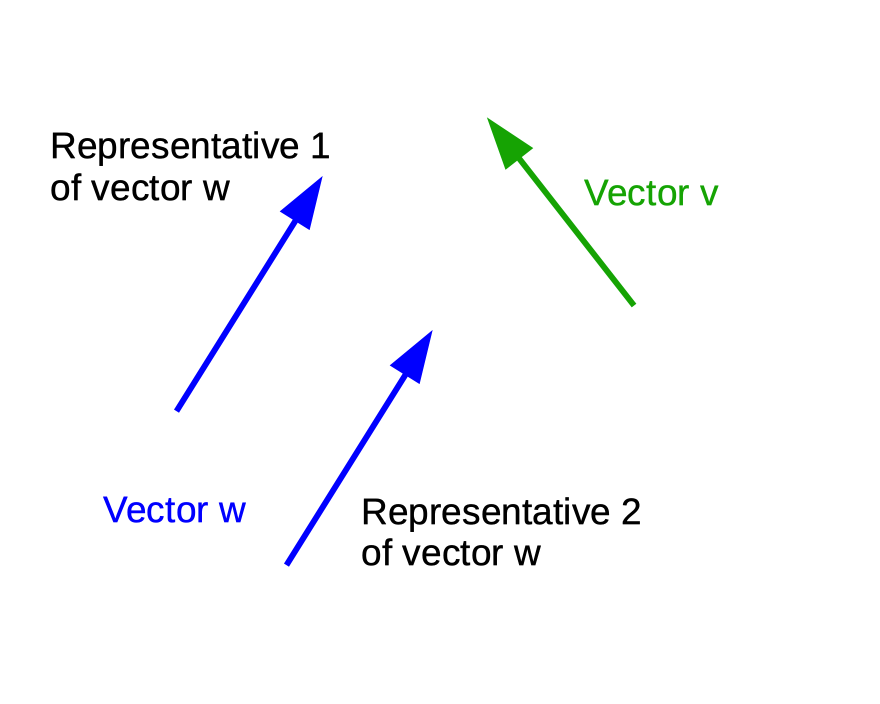
\includegraphics[width=12.22in,]{odg/vector-physics-perspective}

\hypertarget{intro-linalg-computer-science-perspective}{%
\subsection{Computer Science Perspective}\label{intro-linalg-computer-science-perspective}}

In the computer science perspective vectors are ordered list of numbers. Later we will see that vectors can also contain more general objects like strings. As an example, we assume that we are analyzing carcasses and the only thing we know about a carcass is its slaughter-weight (SW) and its price (P). The different carcasses can then be represented by a pair of numbers the first being the slaughter-weight and the second being the price. It is important to note here, that the order of the number matters. In terms of vectors, here each carcass is represented by a two-dimensional vector.

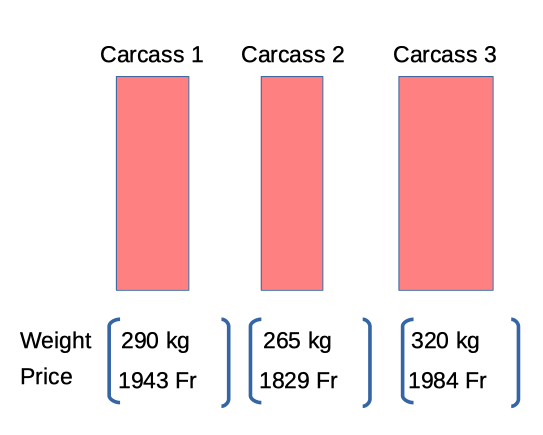
\includegraphics[width=7.54in,]{odg/vector-cs-perspecitve}

\hypertarget{intro-linalg-geometric-context}{%
\subsection{Geometric Context}\label{intro-linalg-geometric-context}}

Some basic properties of vectors are introduced using the geometric context, that a vector is an arrow located in a certain coordinate system with its tail sitting at the origin of the coordinate system. This is a little bit different from the physics perspective (see \ref{intro-linalg-physics-perspective}) where the arrow can sit anywhere in space. In linear algebra it is almost always the case that vectors are rooted at the origin. Once we understand the properties of vectors in the context of arrows in space, we can then translate these properties to the list-of-numbers point of view (see \ref{intro-linalg-computer-science-perspective}) considering the coordinates of the vectors.

\hypertarget{intro-linalg-coordinate-system}{%
\subsection{Coordinate System}\label{intro-linalg-coordinate-system}}

It is important to introduce the coordinate system, because this will be the basis of the correspondence between the two perspectives of linear algebra. For the moment, we focus on two dimensions. The horizontal line is called the x-axis and the vertical line is called the y-axis. The place where the two lines intersect is called the origin. An arbitrary length is chosen to represent \(1\). The coordinates of a vector is a pair of numbers that give instructions for how to get from the tail of that vector at the origin to its tip. The first number tells you how far to walk along the x-axis (positive numbers indicating rightward motion, negative numbers indicating leftward motion) and the second number tell you how far to walk parallel to the y-axis (positive numbers indicating upward motion, negative numbers indicating downward motion).

\begin{figure}[!ht]
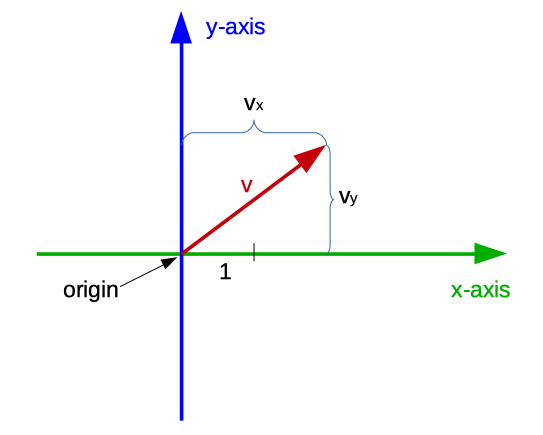
\includegraphics[width=1\linewidth,]{odg/coordinate-system} \caption{Coordinate System}\label{fig:coordinate-system}
\end{figure}

\hypertarget{intro-linalg-vector-operations}{%
\subsection{Vector Operations}\label{intro-linalg-vector-operations}}

The vectors by themselves can be pretty interesting objects, but they get really useful when considering some operations that we can perform on them. Here we consider three basic operations.

\begin{enumerate}
\def\labelenumi{\arabic{enumi}.}
\tightlist
\item
  addition
\item
  multiplication by a scalar number and
\item
  dot product
\end{enumerate}

\hypertarget{intro-linalg-vector-addition}{%
\subsubsection{Addition}\label{intro-linalg-vector-addition}}

Let us assume, we have two vectors \(v\) and \(w\). To add these two vectors, move the second one such that its tail sits at the tip of the first one. Then draw a new vector from the tail of the first one to the tip of the second one. The new vector corresponds to the sum of the two vectors (Figure \ref{fig:vector-sum}).

\begin{figure}[!ht]
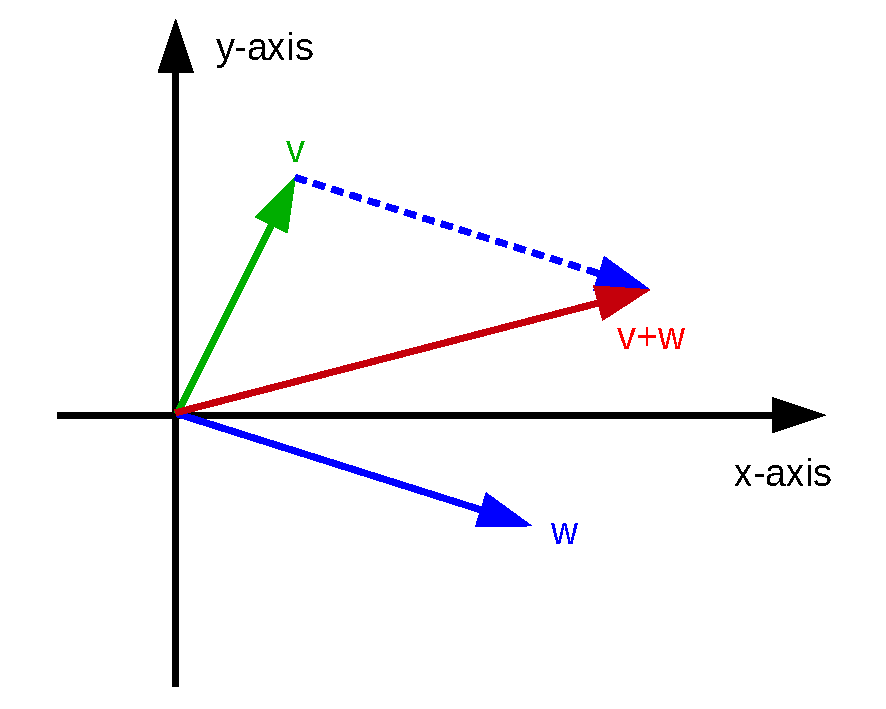
\includegraphics[width=1\linewidth,]{odg/vector-sum} \caption{Addition of two vectors}\label{fig:vector-sum}
\end{figure}

Numerically, vector addition corresponds to summing up each of the coordinates individually. Hence if we have two vectors \(v\) and \(w\) with their coordinates given as

\[v = \left[\begin{array}{c} v_x \\ v_y \end{array}\right] \text{, } w = \left[\begin{array}{c} w_x \\ w_y \end{array}\right]\]

then the sum \(v+w\) has coordinates

\[v+w =  \left[\begin{array}{c} v_x + w_x \\ v_y+w_y \end{array}\right]\]

\hypertarget{intro-linalg-vector-scalar-multiplication}{%
\subsubsection{Multiplication by a Scalar Number}\label{intro-linalg-vector-scalar-multiplication}}

This operation is best understood by looking at a few examples. If we take the number \(2\) and multiply it by a certain vector \(v\), this means that we stretch out the vector \(v\) such that it is \(2\) times as long as the original vector. Multiplication of a vector with positive numbers does not change the direction of the vector. Multiplying a vector \(v\) with a negative number like \(-0.5\) then the direction gets flipped around and then squished by \(0.5\).

\begin{figure}[!ht]
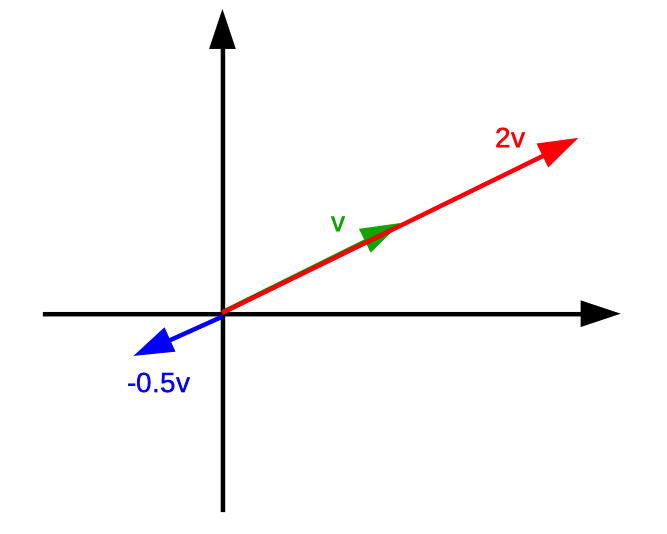
\includegraphics[width=1\linewidth,]{odg/vector-scalar-multiplication} \caption{Scalar Multiplication of Vectors}\label{fig:vector-scalar-multiplication}
\end{figure}

The operation of multiplying a vector by a given number, like \(2\) or \(-0.5\) is also called \textbf{scaling} and that is the reason why in linear algebra the numbers like \(2\) and \(-0.5\) are called \textbf{scalar} numbers or just scalars. Numerically, stretching a vector by a given number like \(2\), corresponds to multiplying each of the coordinate components by that factor \(2\). For a vector \(v\) with coordinate components \(v_x\) and \(v_y\), the vector \(2v\) has coordinates \(2v_x\) and \(2v_y\)

\[v = \left[\begin{array}{c} v_x \\ v_y \end{array}\right] \text{, }\quad 2v = \left[\begin{array}{c} 2v_x \\ 2v_y \end{array}\right]\]

\hypertarget{intro-linalg-dot-product}{%
\subsubsection{Dot Product}\label{intro-linalg-dot-product}}

The dot product is explained in a different video that can be seen on \url{https://youtu.be/LyGKycYT2v0}. Numerically, if you have two vectors of the same dimension, meaning two lists of numbers of the same length, e.g.~\(v\) and \(w\) then their dot product \(v \cdot w\) can be computed by pairing up all of the coordinates, multiplying these pairs together and adding the result. So the vectors

\[v = \left[\begin{array}{c} v_x \\ v_y \end{array}\right] \text{ and } w= \left[\begin{array}{c} w_x \\ w_y \end{array}\right]\]

their dot product \(v \cdot w\) then is computed as

\[v \cdot w = v_x * w_x + v_y * w_y\]

\hypertarget{intro-linalg-matrices}{%
\section{Matrices}\label{intro-linalg-matrices}}

The introduction to the topic of matrices is available from \url{https://youtu.be/kYB8IZa5AuE} and \url{https://youtu.be/XkY2DOUCWMU}. An \(m \times n\) matrix is a table-like object of \(m*n\) numbers arranged in \(m\) rows and \(n\) columns. In general the \(m \times n\) matrix \(A\) has the following structure.

\[
A = \left[
\begin{array}{cccc}
a_{11}  &  a_{12} &  \ldots  &  a_{1n} \\
a_{21}  &  a_{22} &  \ldots  &  a_{2n} \\
\vdots  &         &          &  \vdots \\
a_{m1}  &  a_{m2} &  \ldots  &  a_{mn}
\end{array}
\right]
\]

The \(m*n\) numbers inside of the square brackets are called elements of the matrix. The element of matrix \(A\) that is in row \(i\) and in column \(j\) is called \(a_{ij}\) or \((A)_{ij}\). As an example

\[
A =  \left[
\begin{array}{ccc}
2  &  3  &  1  \\
5  &  1  &  2
\end{array}
\right]
\]
is a \(2 \times 3\) matrix. In the first row the second element corresponds to \((A)_{12} = a_{12} = 3\). An \(n\times n\) matrix (i.e.~a matrix with equal numbers of rows and columns) is called a \textbf{quadratic} matrix. Two matrices \(A\) and \(B\) are called \textbf{equal}, if they have the same number of rows and columns and if the corresponding elements are the same, i.e.

\[
(A)_{ij} = (B)_{ij} \text{ for all i and j}
\]

\hypertarget{intro-linalg-special-matrices}{%
\subsection{Special Matrices}\label{intro-linalg-special-matrices}}

The following matrices are special and are used in special cases.

\begin{itemize}
\tightlist
\item
  \textbf{Nullmatrix}: The \(m\times n\) matrix \(0\) is called Nullmatrix, if each element is equal to zero.
\item
  \textbf{Upper Triangular Matrix}: The square matrix \(R\) is called upper triangular matrix, if \((R)_{ij} = 0\) for \(i>j\).
\item
  \textbf{Lower Triangular Matrix}: The square matrix \(L\) is called lower triangular matrix, if \((L)_{ij} = 0\) for \(i<j\).
\item
  \textbf{Diagonal Matrix}: The square matrix \(D\) is called diagonal matrix, if \((D)_{ij} = 0\) for \(i\ne j\).
\item
  \textbf{Identity Matrix}: The diagonal matrix \(I\) is called identity matrix, if all diagonal elements \((I)_{ii} = 1\).
\item
  \textbf{Column Vector}: A \(m\times 1\) matrix is often called a column vector.
\item
  \textbf{Row Vector}: A \(1\times n\) matrix is is often called a row vector.
\end{itemize}

\hypertarget{intro-linalg-matrix-operation}{%
\subsection{Matrix Operations}\label{intro-linalg-matrix-operation}}

The following operations with matrices are defined.

\hypertarget{intro-linalg-matrix-addition}{%
\subsubsection{Addition}\label{intro-linalg-matrix-addition}}

For two \(m\times n\) matrices \(A\) and \(B\), their sum \(A+B\) is again a \(m\times n\) matrix with each element corresponding to the sum of the corresponding elements from \(A\) and \(B\). Hence, we can write

\[(A+B)_{ij} = (A)_{ij} + (B)_{ij} \text{ for all i and j}\]

\hypertarget{intro-linalg-matrix-multiplication-with-number}{%
\subsubsection{Multiplication with a Number}\label{intro-linalg-matrix-multiplication-with-number}}

A \(m\times n\) matrix A is multiplied by a number \(\alpha\) by multiplying every element \((A)_{ij}\) of \(A\) with \(\alpha\). The result \(\alpha * A\) is computed as \((\alpha * A)_{ij} = \alpha * (A)_{ij}\) for all \(i\) and \(j\).

\hypertarget{intro-linalg-multiplication-two-matrices}{%
\subsubsection{Multiplication of two Matrices}\label{intro-linalg-multiplication-two-matrices}}

Given a \(m\times n\) matrix \(A\) and a \(n\times p\) matrix \(B\), their matrix product \(AB\) is a \(m\times p\) matrix with

\[ (AB)_{ij} = \sum_{k=1}^n (A)_{ik} * (B)_{kj} = (A)_{i1} * (B)_{1j} + (A)_{i2} * (B)_{2j} + \ldots + (A)_{in} * (B)_{nj}\]

\hypertarget{intro-linalg-laws-matrix-operations}{%
\subsubsection{Laws of Matrix Operations}\label{intro-linalg-laws-matrix-operations}}

\begin{itemize}
\tightlist
\item
  \textbf{Commutativity}: For two \(m\times n\) matrices \(A\) and \(B\) the addition is commutative, i.e.~\(A + B = B + A\).
\item
  \textbf{Associativity of addition}: For \(m\times n\) matrices \(A\), \(B\) and \(C\), the addition is associative, i.e., \(A + (B + C) = (A + B) + C\)
\item
  \textbf{Associativity of multiplication}: For a \(m\times n\) matrix \(A\), a \(n \times p\) matrix \(B\) and a \(p \times q\) matrix \(C\), the multiplication is associative, i.e., \(A(BC) = (AB)C\)
\item
  \textbf{Distributivity}: For \(m\times n\) matrices \(A\) and \(B\) and \(n\times p\) matrices \(C\) and \(D\), the distributive law holds, i.e., \((A+B)C = AC + BC\) and \(A(C + D) = AC + AD\)
\end{itemize}

\hypertarget{intro-linalg-laws-matrix-transpose}{%
\subsubsection{Matrix Transpose}\label{intro-linalg-laws-matrix-transpose}}

Given a \(m\times n\) matrix \(A\), then the \(n\times m\) matrix \(A^T\) is called its \textbf{transpose}, if \((A^T)_{ij} = A_{ji}\). The matrix \(A\) is called \textbf{symmetric}, if \(A = A^T\). For every matrix \(A\) the transpose of the transpose is the matrix itself, i.e., \((A^T)^T = A\). For any \(m\times n\) matrices \(A\) and \(B\), the transpose \((A+B)^T\) of their sum \((A+B)\) is computed as

\[(A+B)^T = A^T + B^T\]

For every \(m\times n\) matrix \(A\) and every \(n\times p\) matrix \(B\), it holds that

\[(AB)^T = B^T A^T\]

\hypertarget{intro-linalg-inverse-matrix}{%
\subsubsection{Inverse of a Matrix}\label{intro-linalg-inverse-matrix}}

In this section, we are looking at square matrices. The \textbf{inverse} \(X\) of a square matrix \(A\) is defined as the square matrix that satisfies the condition \(AX = I\). If the inverse matrix \(X\) exists, then the matrix \(A\) is called invertable. If \(X\) does not exist, \(A\) is called singular. If the inverse of a matrix \(A\) exists, it is uniquely determined and we call it \(A^{-1}\).

Let us assume two invertable \(n\times n\) matrices \(A\) and \(B\), then the following equations hold

\begin{enumerate}
\def\labelenumi{\arabic{enumi}.}
\tightlist
\item
  \(A^{-1}A = I\)
\item
  \(A^{-1}\) is invertable and \((A^{-1})^{-1} = A\)
\item
  \(I\) is invertable and \(I^{-1} = I\)
\item
  \(AB\) is invertable and \((AB)^{-1} = B^{-1}A^{-1}\)
\item
  \(A^T\) is invertable and \((A^T)^{-1} = (A^{-1})^T\)
\end{enumerate}

For every square matrix \(A\), the following statements are equivalent.

\begin{enumerate}
\def\labelenumi{\arabic{enumi}.}
\tightlist
\item
  \(A\) is invertable
\item
  The system of equations \(Ax = b\) is solvable for every \(b\).
\item
  The system of equations \(Ax = 0\) has only the trivial solution \(x=0\).
\end{enumerate}

\hypertarget{intro-linalg-orthogonal-matrix}{%
\subsubsection{Orthogonal Matrices}\label{intro-linalg-orthogonal-matrix}}

A square matrix \(A\) is called \textbf{orthogonal}, if the condition \(A^TA = I\) holds. For two orthogonal matrices \(A\) and \(B\), the following statements hold.

\begin{enumerate}
\def\labelenumi{\arabic{enumi}.}
\tightlist
\item
  \(A\) is invertable and \(A^{-1} = A^T\)
\item
  \(A^{-1}\) is orthogonal
\item
  \(AB\) is orthogonal
\item
  \(I\) is orthogonal
\end{enumerate}

\hypertarget{intro-linalg-systems-of-equations}{%
\section{Systems Of Equations}\label{intro-linalg-systems-of-equations}}

Systems of linear equations are introduced based on \citep{Nipp2002} and \citep{Searle1971}. Solving systems of linear equations is one of the fundamental tasks of linear algebra. We start with a general example of a system of linear equations which is given as

\begin{align}
 x_1 + 2x_2 &= 5 \notag \\
2x_1 + 3x_2 &= 8
\label{eq:intro-linalg-first-example}
\end{align}

In \eqref{eq:intro-linalg-first-example} we are given a system of linear equations with two equations and two unknowns \(x_1\) and \(x_2\). The aim is to find numeric values for \(x_1\) and \(x_2\) such that both equations are satisfied. Inserting the values \(x_1 = 1\) and \(x_2 = 2\) into the above equations show that they are both satisfied. Hence the set \(L = \{x_1 = 1, x_2 = 2\}\) consisting of the values for \(x_1\) and \(x_2\) that satisfy both equations is called a solution or a solution set for the above shown equations.

In general, a linear system of equations consists of \(m\) equations and \(n\) unknowns. In the example \eqref{eq:intro-linalg-first-example}, \(m=2\) and \(n=2\).

The example in \eqref{eq:intro-linalg-no-solution} does not have any solutions.

\begin{align}
 x_1 +  x_2 &= 4 \notag \\
2x_1 + 2x_2 &= 5
\label{eq:intro-linalg-no-solution}
\end{align}

This can be seen, that if the first equation in \eqref{eq:intro-linalg-no-solution} is multiplied by \(2\), we get \(2x_1 + 2x_2 = 8\) which contradicts the second equation shown in \eqref{eq:intro-linalg-no-solution}.

A system with \(m=2\) equations and \(n=3\) unknowns in shown in \eqref{eq:intro-linalg-infnr-solution}.

\begin{align}
 x_1 -  x_2 +  x_3 &= 2 \notag \\
2x_1 +  x_2 -  x_3 &= 4  
\label{eq:intro-linalg-infnr-solution}
\end{align}

There are infinitely many solutions consisting of \(x_1 = 2\), \(x_2 = \alpha\) and \(x_3 = \alpha\) for any real number \(\alpha\).

The examples in \eqref{eq:intro-linalg-first-example}, \eqref{eq:intro-linalg-no-solution} and \eqref{eq:intro-linalg-infnr-solution} already show all possible cases that may occur when solving linear systems of equations. The question is how to determine the set of all solutions of a system of linear equations.

\hypertarget{intro-linalg-matrix-vector-notation}{%
\subsection{Matrix-Vector Notation}\label{intro-linalg-matrix-vector-notation}}

So far, we have written systems of linear equations explicitly in the sense that every equation was written on one line. For small systems this is not a problem. But when the number of equations (\(m\)) and the number of unknowns (\(n\)) get very large, the explicit notation is no longer feasible. Hence, we need a notation that can also be used for large systems of equations. The so-called matrix-vector notation provides an efficient way to write down large systems of equations very efficiently.

We return to the example given by \eqref{eq:intro-linalg-first-example} and we define the matrix \(A\) to be

\[
A = \left[
\begin{array}{cc}
1  &  2 \\
2  &  3
\end{array}
\right], 
\]

the vector \(x\) to be

\[
x = \left[
\begin{array}{c}
x_1  \\
x_2  
\end{array}
\right], 
\]

and the vector \(y\) to be

\[
y = \left[
\begin{array}{c}
5  \\
8  
\end{array}
\right], 
\]

With these definitions, we can write the system of equations given in \eqref{eq:intro-linalg-first-example} using matrix-vector notation as

\begin{equation}
A \cdot x = y
\label{eq:intro-linalg-matrix-vector-notation}
\end{equation}

\hypertarget{intro-linalg-solving-systems-of-linear-equations}{%
\section{Solving Systems of Linear Equations}\label{intro-linalg-solving-systems-of-linear-equations}}

If matrix \(A\) in \eqref{eq:intro-linalg-matrix-vector-notation} is not singular, i.e.~the inverse Matrix \(A^{-1}\) of \(A\) does exist, the solution \(x\) to \eqref{eq:intro-linalg-matrix-vector-notation} can be written as \(x = A^{-1}y\). This result is obtained by pre-multiplying both sides of \eqref{eq:intro-linalg-matrix-vector-notation} with \(A^{-1}\) and since a matrix times its inverse results in the identity matrix \(I\), the solution is obtained as

\begin{align}
            A \cdot x  &=  y \notag \\
A^{-1}\cdot A \cdot x  &=  A^{-1} \cdot y \notag \\
            I \cdot x  &=  A^{-1} \cdot y \notag \\
                    x  &=  A^{-1} \cdot y
\label{eq:intro-linalg-matrix-vector-notation-solution-derivation}
\end{align}

For systems of equations with a singular matrix \(A\), solutions can be found, if the equations are \textbf{consistent}. The linear equations \(Ax = y\) are consistent, if any linear relationship existing among the rows of \(A\) also exist among the corresponding elements of \(y\). As a simple example, the equations

\[
\left[
\begin{array}{cc}
1  &  2  \\
3  &  6
\end{array}\right]
\left[
\begin{array}{c}
x_1  \\
x_2
\end{array}\right]
=
\left[
\begin{array}{c}
7  \\
21
\end{array}\right]
\]
are consistent. In the matrix on the left the second row corresponds to three times the first row and in the vector on the right, the second element is also three times the first element. In contrast the equations

\[
\left[
\begin{array}{cc}
1  &  2  \\
3  &  6
\end{array}\right]
\left[
\begin{array}{c}
x_1  \\
x_2
\end{array}\right]
=
\left[
\begin{array}{c}
7  \\
24
\end{array}\right]
\]
are not consistent. From this example, we can already see that non-consistent equations do not have any solutions. But consistent equations \(Ax = y\) have a solution which can be written as \(x = Gy\) if and only if, \(AGA = A\) which means that \(G\) is a so-called generalized inverse of \(A\). The matrix \(G\) is often written as \(A^-\). The proof of this statement is given on page 9 of \citep{Searle1971}.

\hypertarget{intro-rstats}{%
\chapter{Introduction To R and RStudio}\label{intro-rstats}}

According to the website \url{https://www.r-project.org/}, R \citep{RCoreTeam2018} is a free software environment for statistical computing and graphics. Because R is free and it is available for the most commonly used operating systems such as Windows, MacOsX and Linux, it has become very popular in statistics and in data science. Furthermore, R can be extended with user-contributed code and documentation (called R-packages) in a very easy and standardised way. The number of available R-packages is growing rapidly and has reached

RStudio (\url{https://www.rstudio.com/}) is a private company that among a large number of different products distributes the RStudio Integrated Development Environment (IDE) for R. A great number of different resources about R and RStudio IDE is available. Some of them are listed here.

\begin{itemize}
\tightlist
\item
  \textbf{R}: From the R website, there is an introduction to R available at: \url{https://cran.r-project.org/doc/manuals/r-release/R-intro.html}.
\item
  \textbf{RStudio IDE}: The link \url{https://resources.rstudio.com/} points to a series of webinars introducing R and RStudio.
\end{itemize}

  \bibliography{lbgfs2021.bib}

\end{document}
